%; whizzy chapter -dvi
% -initex iniptex -latex platex -format platex -bibtex jbibtex -fmt fmt
% 以上 whizzytex を使用する場合の設定。

%     Tokyo Debian Meeting resources
%     Copyright (C) 2012 Junichi Uekawa
%     Copyright (C) 2011 Nobuhiro Iwamatsu

%     This program is free software; you can redistribute it and/or modify
%     it under the terms of the GNU General Public License as published by
%     the Free Software Foundation; either version 2 of the License, or
%     (at your option) any later version.

%     This program is distributed in the hope that it will be useful,
%     but WITHOUT ANY WARRANTY; without even the implied warranty of
%     MERCHANTABILITY or FITNESS FOR A PARTICULAR PURPOSE.  See the
%     GNU General Public License for more details.

%     You should have received a copy of the GNU General Public License
%     along with this program; if not, write to the Free Software
%     Foundation, Inc., 51 Franklin St, Fifth Floor, Boston, MA  02110-1301 USA

%  preview (shell-command (concat "evince " (replace-regexp-in-string "tex$" "pdf"(buffer-file-name)) "&"))
% 画像ファイルを処理するためにはebbを利用してboundingboxを作成。
%(shell-command "cd image201201; ebb *.png")

%%ここからヘッダ開始。

\documentclass[mingoth,a4paper]{jsarticle}
\usepackage{monthlyreport}

% 日付を定義する、毎月変わります。
\newcommand{\debmtgyear}{2013}
\newcommand{\debmtgmonth}{1}
\newcommand{\debmtgdate}{13}
% started from zero:
% (let ((year 2013) (month 1)) (+ (* (- year 2005) 12) month -1))
\newcommand{\debmtgnumber}{96}

\begin{document}

\begin{titlepage}
\thispagestyle{empty}
% タイトルページ:編集必要な部分は最初のマクロに飛ばすこと

\vspace*{-2cm}
第\debmtgnumber{}回 東京エリア Debian 勉強会資料\\
\hspace*{-2cm}

\includegraphics{image2012-natsu/dotdeb.pdf}\\
\hfill{}\debmtgyear{}年\debmtgmonth{}月\debmtgdate{}日

% ここはアップデートすること
% 全角文字にしないとフォントのサイズが合わないので注意
\rotatebox{10}{\fontsize{32}{32} {\gt 特集1: 2013年度計画}}

\rotatebox{10}{\fontsize{32}{32} {\gt 特集2: アンケート集計}}

\vspace*{-2cm}
\hfill{}
\includegraphics[height=6cm]{image200502/openlogo-nd.eps}
\end{titlepage}

\dancersection{Introduction}{上川 純一}

\begin{multicols}{2}
 

 今月のDebian勉強会へようこそ。これからDebianの世界にあしを踏み入れると
 いう方も、すでにどっぷりとつかっているという方も、月に一回Debianについ
 て語りませんか?

 Debian勉強会の目的は下記です。

 \begin{itemize}
 \item \underline{Debian Developer} (開発者)の育成。
 \item 日本語での「\underline{開発に関する情報}」を整理してまとめ、アップデートする。
 \item \underline{場}の提供。
 \begin{itemize}
  \item 普段ばらばらな場所にいる人々が face-to-face で出会える場を提供
	する。
  \item Debian のためになることを語る場を提供する。
  \item Debianについて語る場を提供する。
 \end{itemize}
 \end{itemize}		

 Debianの勉強会ということで究極的には参加者全員がDebian Packageをがりがり
 と作るスーパーハッカーになった姿を妄想しています。情報の共有・活用を通し
 て Debianの今後の能動的な展開への土台として、「場」としての空間を提供す
 るのが目的です。

\end{multicols}

\newpage

\begin{minipage}[b]{0.2\hsize}
 \definecolor{titleback}{gray}{0.9}
 \colorbox{titleback}{\rotatebox{90}{\fontsize{80}{80} {\gt デビアン勉強会} }}
\end{minipage}
\begin{minipage}[b]{0.8\hsize}
\hrule
\vspace{2mm}
\hrule
\begin{multicols}{2}
\tableofcontents
\end{multicols}
\vspace{2mm}
\hrule
\end{minipage}

\dancersection{事前課題}{上川純一}

今回の事前課題は以下です:
\begin{enumerate}
 \item 2013年の勉強会で発表したい内容を教えてください。
 \item 2015年では Debianはどうなっているかを大胆に予想してください。
\end{enumerate}
この課題に対して提出いただいた内容は以下です。
\begin{multicols}{2}
{\small
 %; whizzy-master ../debianmeetingresume201301.tex
% $B0J>e$N@_Dj$r$7$F$$$k$?$a!"$3$N%U%!%$%k$G(B M-x whizzytex $B$9$k$H!"(B
% whizzytex$B$,MxMQ$G$-$^$9(B

\begin{prework}{$B>e@n=c0l(B}

\preworksection{2013$BG/$NJY6/2q$GH/I=$7$?$$FbMF$r65$($F$/$@$5$$(B}
\preworksection{2015$BG/$G$O(BDebian$B$,$I$&$J$C$F$$$k$+$rBgC@$KM=A[$7$F$/$@$5$$(B}


\end{prework}

}
\end{multicols}

\dancersection{Debian Trivia Quiz}{野島 貴英}

ところで、みなさん Debian 関連の話題においついていますか?Debian関連の話
題はメーリングリストをよんでいると追跡できます。ただよんでいるだけではは
りあいがないので、理解度のテストをします。特に一人だけでは意味がわからな
いところもあるかも知れません。みんなで一緒に読んでみましょう。

今回の出題範囲は\url{debian-devel-announce@lists.debian.org} や \url{debian-devel@lists.debian.org}に投稿された
内容とDebian Project Newsからです。

\begin{multicols}{2}
%; whizzy-master ../debianmeetingresume201211.tex
% $B0J>e$N@_Dj$r$7$F$$$k$?$a!"$3$N%U%!%$%k$G(B M-x whizzytex $B$9$k$H!"(Bwhizzytex$B$,MxMQ$G$-$^$9!#(B
%

\santaku
{wiki.debian.org$B$G;H$o$l$F$$$?(Bwiki$B%7%9%F%`$N%=%U%H%&%'%"$NL>A0$O!)(B}
{pukiwiki}
{mine}
{moin}
{C}
{$B@?$K0d48$J$,$i!"(Bwiki.debian.org$B$,$3$NA0%/%i%C%/$5$l$?$h$&$G$9!#(B
$BB>$GF1$8EPO?%a!<%k%"%I%l%9$H%Q%9%o!<%I$NAH$r;H$C$F$$$k?M$O!"(B
$B$9$0$K%Q%9%o!<%I$rJQ$($?J}$,$h$$$G$7$g$&!#(B}

\santaku
{$B5nG/$NG/Kv$N(Bpopcon$BD4::$G(BNo.1$B$K51$$$?%W%i%C%H%U%)!<%`$O!)(B}
{$BEvA3(Barmel$B$@$m!)(B}
{i386}
{amd64}
{C}
{\url{http://popcon.debian.org/}$B$N%H%C%W%Z!<%8$K7k2L$N%0%i%U$,$"$j$^$9!#(B
 $B:#$^$G(BNo.1$B$r7h$a$F$$$?(Bi386$B$rG/Kv$G(Bamd64$B$,H4$-5n$C$?$h$&$G$9!#(B}

\santaku
{1$B7nF,$N(BDPN$B$GJs9p$N$"$C$?!"(Bwheezy$B$K;D$C$F$$$k(BRC$B%P%0$N?t$O(B1$B7n(B5$BF|;~E@$G$"$H2?8D!)(B}
{$B$"$H(B321$B8D(B}
{$B$"$H(B171$B8D(B}
{$B$"$H(B17$B8D(B}
{B}
{$B4JC1$KD>$;$k(B/$BB><#$l$P>!<j$K<#$j$=$&$b$N$r4^$s$G(B171$B8D!#<j$,$+$+$j$=$&$J$N$O(B
$B$@$$$?$$(B116$B8D$@$=$&$G$9!#(B}

\santaku
{$B:#G/(Bamazon$B$+$i(BDebian Project$B$X$$$/$i$+$N(BAWS$B$NMxMQ7t$r%9%]%s%5!<$7$F$b$i$C$?$=$&$J$N$G$9$,!"6b3[$K$9$k$H$*$$$/$i!)(B}
{8000USD}
{800USD}
{80000USD}
{A}
{$BF|K\1_$K$9$k$HLs(B72$BK|1_J,$NMxMQ7t!#(BQA$B$K$O==J,$H$N$3$H$G$7$?!#(B}











\end{multicols}

\dancersection{最近のDebian関連のミーティング報告}{上川純一}
\subsection{東京エリアDebian勉強会95回目報告}
% (query-replace-regexp "<.*?>" "")
% (query-replace-regexp "^[	 ]\+" "")

2012年12月のDebian勉強会はあんさんぶる荻窪で開催されました。
参加者はキタハラさん、野首さん、dictossさん、sudouさん、青木さん、
koedoyoshidaさん、野島さん、石井さん、yy\_y\_ja\_jpさん、seiji-nさん、
yamamotoさん、上川でした。

最初に事前課題の紹介を行いました。
DFSGに対しての熱い意気込みを感じられました。

上川が2012年のDebian勉強会で何をやったかについて紹介しました。
Debian開発者の興味のある内容を偏った感じでカバーしているという印象です。
来年はもっと幅広いテーマをとりあげてもいいかもしれません。

上川は最近の法律とか動向とかについて思うことを議論しました。
特に結論はないですが、危機感を共有できたら幸いです。

青木さんがim-config について紹介しました。
現役の漢字入力の方法が何種類もあるということに新たな驚きを感じました。

%-------------------------------------------------------------------------------
\dancersection{Debian勉強会予約システムアンケート集計}{上川 純一}
%-------------------------------------------------------------------------------
\index{Debianべんきょうかいよやくしすてむ@Debian勉強会予約システム}
\index{あんけーと@アンケート}
\index{R}

\subsection{アンケート集計結果の処理}

東京エリアDebian勉強会ではアンケートをとっています。集計結果を眺めてみま
しょう。データはDebian勉強会予約システムのアンケート出力インタフェース
\url{http://debianmeeting.appspot.com/enquete/showallresults}から取得し
ます\footnote{取得したファイルを \url{image201301/enquete.csv} において
おきます。}
出力形式は各行がDebian勉強会予約システムに登録している個人で、各列がそれ
ぞれのセッションです。各コラム名は一意なキーとして扱えるようにするためイベン
ト名とセッション名を足してかつイベントのハッシュ値の一部を追加したものを
採用しています。

R で処理するためにデータを読み込み前処理を行うのには便利なスクリプトを用
意しているのでそれを利用します。

\begin{commandline}
> source('getenquete.R')
\end{commandline}

まず全体的なスコアのつき方から紹介しましょう。
\fgref{fig:enquete-score-distribution}にすべてのお題のスコアの分布を並べ
ています。時系列にならんではいますがそれぞれのテーマごとに並んでいるので
時系列とは限りません。

\fgref{fig:all-enquete-score-distribution}に平均点がどういう分布をしてい
るのかを図示しています。八割くらいは4点になり、一割づつ5点と3点があるよう
なスコア分布であることが見て取れます。特にひどいときには平均点が2点になっ
てるような気もします。ここから読み取れる全体的な傾向としては、ほとんどの場合は平均点で、特によいときに
は良い点数、特に悪い時には悪い点数をつけている人が多いということでしょう
か。

\begin{figure}[h]
\begin{center}
  \includegraphics[width=0.8\hsize,angle=270]{image201301/enquete_boxplot.eps}

\end{center}
 \caption{毎回のスコアの分布}\label{fig:enquete-score-distribution}
\end{figure}


\begin{figure}[h]
\begin{center}
 \includegraphics[width=0.8\hsize,angle=270]{image201301/raw_average_score_density.eps}

 \caption{すべての回を通しての平均点の分布}
 \label{fig:all-enquete-score-distribution}
\end{center}
\end{figure}

データの癖を確認するために代表的なユーザの例を見てみます。
\fgref{fig:example-user-score-1}\fgref{fig:example-user-score-2}にどのス
コアを何度つけたのかをグラフにしています。ほとんどの場合は4をつけて、一
部に5、3をつけ、2と1はほとんどつけてないという結果になっています。こ
れに数回しか評価に参加していないユーザが4をつけるなどのバイアスが加わっ
て全体としては4がさらに強調されているような気もします。

\begin{figure}[h]
\begin{center}
 \includegraphics[width=0.8\hsize,angle=270]{image201301/score_hist_8.eps}

 \caption{あるユーザのつけたスコア分布}
 \label{fig:example-user-score-1}
\end{center}
\end{figure}

\begin{figure}[h]
\begin{center}
 \includegraphics[width=0.8\hsize,angle=270]{image201301/score_hist_9.eps}

 \caption{また別のユーザのつけたスコア分布}
 \label{fig:example-user-score-2}
\end{center}
\end{figure}

気になるのでセッションの具体例をみてみましょう。2010年12月の勉強会のDebian Miniconf企画
会議はぐだぐだだったので仕方がないでしょう。一方、
2012年1月の事前課題紹介に辛口の評価が多かったのが気になります。n=4 なのでそん
なに少数派でもないようです。今から振り返ってもいまいちぱっとしない内容な
のですが運営がまずかったのでしょうか。

\begin{commandline}
> raw_average_score[!is.na(raw_average_score) & raw_average_score < 3]
                第71回東京エリアDebian勉強会.2010年12月勉強会.Debian.Miniconf.企画.2eca 
                                                                               2.333333 
              第84回東京エリアDebian勉強会.2012年1月勉強会.事前課題紹介.2012年企画.f447 
                                                                               2.500000 
第84回東京エリアDebian勉強会.2012年1月勉強会.第3回月刊Debhelper.dh_auto_..dh_build.f447 
                                                                               2.500000 
> enquete_response[!is.na(raw_average_score) & raw_average_score < 3]
                第71回東京エリアDebian勉強会.2010年12月勉強会.Debian.Miniconf.企画.2eca 
                                                                                      6 
              第84回東京エリアDebian勉強会.2012年1月勉強会.事前課題紹介.2012年企画.f447 
                                                                                      4 
第84回東京エリアDebian勉強会.2012年1月勉強会.第3回月刊Debhelper.dh_auto_..dh_build.f447 

> scaled_average_score['第84回東京エリアDebian勉強会.2012年1月勉強会.事前課題紹介.2012年企画.f447']
第84回東京エリアDebian勉強会.2012年1月勉強会.事前課題紹介.2012年企画.f447 
                                                                -1.289405 
                                                                                      4 
\end{commandline}

一方でハイスコア側を眺めてみましょう。最高のスコアは「第79回東京エリア
Debian勉強会.2011年8月勉強会.Debianパッケージのビルド方法」と「第91回東京
エリアDebian勉強会.2012年8月勉強会.月刊.Debhelper.共有ライブラリ編」です。
それぞれn=2とn=3で全員最高点を指定した結果です。アンケートに回答してくれ
た人数が少ないのが気になりますが、力作で聞いてておもしろいものでした。
「第72回東京エリアDebian勉強会.2011年1月勉強会.Kinect」$ 4.875 (sd=0.35,
n=8)$ と「第95回東京エリアDebian勉強会.2012年12月勉強会.著作権法改正」
$4.75 (sd=0.5, n=4)$ が比較的投票数も高くてスコアの高いものです。Kinectは
デモ満載でやっていることもぶっ飛んでました。著作権法改正については問題意
識を刺激する内容だったのではないでしょうか。

\begin{commandline}

>  raw_average_score[!is.na(raw_average_score) & raw_average_score > 4.5]
      第71回東京エリアDebian勉強会.2010年12月勉強会.CACertの準備に何が必要か.2eca 
                                                                         4.600000 
       第71回東京エリアDebian勉強会.2010年12月勉強会.俺のlibsaneが火をふくぜ.2eca 
                                                                         4.666667 
                         第72回東京エリアDebian勉強会.2011年1月勉強会.Kinect.f456 
                                                                         4.875000 
   第79回東京エリアDebian勉強会.2011年8月勉強会.Debianパッケージのビルド方法.5dff 
                                                                         5.000000 
            第91回東京エリアDebian勉強会.2012年8月勉強会.DebianでC..11を使う.9796 
                                                                         4.666667 
第91回東京エリアDebian勉強会.2012年8月勉強会.月刊.Debhelper.共有ライブラリ編.9796 
                                                                         5.000000 
                  第95回東京エリアDebian勉強会.2012年12月勉強会.著作権法改正.3f15 
                                                                         4.750000 
> enquete_response[!is.na(raw_average_score) & raw_average_score > 4.5]
      第71回東京エリアDebian勉強会.2010年12月勉強会.CACertの準備に何が必要か.2eca 
                                                                                5 
       第71回東京エリアDebian勉強会.2010年12月勉強会.俺のlibsaneが火をふくぜ.2eca 
                                                                                3 
                         第72回東京エリアDebian勉強会.2011年1月勉強会.Kinect.f456 
                                                                                8 
   第79回東京エリアDebian勉強会.2011年8月勉強会.Debianパッケージのビルド方法.5dff 
                                                                                2 
            第91回東京エリアDebian勉強会.2012年8月勉強会.DebianでC..11を使う.9796 
                                                                                3 
第91回東京エリアDebian勉強会.2012年8月勉強会.月刊.Debhelper.共有ライブラリ編.9796 
                                                                                3 
                  第95回東京エリアDebian勉強会.2012年12月勉強会.著作権法改正.3f15 
                                                                                4 
 
\end{commandline}


\subsection{アンケートの設計について}

今回みられた現象としては、5段階評価の4に評価が集まってしまいました。素
朴にとらえると「よい」といってもらえていることになります。しかしこれだと
分解能が低いと捉えることもできます。

これは「中心化傾向」もしくは
「寛大化傾向」とよばれる現象にあてはまると思います。

アンケート設計の世界ではそれなりにいろいろな対策方法が存在しているようで
すがまだ僕がよく理解できてません。

\clearpage % flush images.

%-------------------------------------------------------------------------------
\dancersection{Debian勉強会2013年度計画}{上川 純一}
%-------------------------------------------------------------------------------
\index{2013ねんどけいかく@2013年度計画}

\subsection{2015年までを妄想する}

{% \tiny
\footnotesize
\begin{tabular}[t]{|p{8em}|p{8em}|p{12em}|p{8em}|p{8em}|}
%\begin{tabular}[t]{|p{8.5em}|p{12em}|p{8em}|p{6em}|p{8em}|}
\hline
2011 &2012 & 2013 & 2014 & 2015 \\
\hline
 %2011

 デスクトップパソコン終了の潮流。

 cpuコア単体では高速化しないように。

 webos終了のお知らせ。

 adobe flash復活のお知らせ(キタ), silverlight終了のお知らせ(台湾を除く)(続いてる?)

 squeezeリリース(おめでとう)

 ipv4割り当ての終了のお知らせ(キタ)

 地上波デジタル移行延長。

 btrfsまだ頑張る(fedora乙)

 java終了(sun java終了)

 open officeがoracle officeに(ナイ)

 &
 %2012

 ノートパソコンよりタブレットのほうが売れている。
 ノートパソコンではmacbookairが常識に。

 ノートパソコンでintelじゃないもの(mips/arm)が主流にはまだならず。タブレッ
 トのほうが主流。

 デスクトップ:ゲーム以外の用途では終了している。

 サーバ:個人レベルではVPS常識。企業ユースでもcloud か、vpsかを自前と比較
     検討する時代。データセンターを置く国を選べる時代。

 携帯電話:
 ガラパゴスの終焉。日本での携帯電話販売でもスマートフォンが50%を超えるように。
     ガラケー向けのネットバンクの提供が終了など、ガラケーからサービスが
     撤退し始める。
 LTE登場、普及しはじめたが、主流になっていない。
 softbankの二年契約はまだ続いている。sim freeへの道は耕されたがあたり前にならなかった。

 btrfsはまだ生き残っているがまだ使われてない?

     openstack で ceph 使う人もいる?

 mysqlからmariadbが派生。

 & 
 % 2013

コンシューマーはノートパソコンを買わなくなった。
ノートパソコンのかわりにスマートフォンを使っている。

スマートフォンが7インチくらいまで拡大、タブレットとは何だったのか。

自宅用のデスクトップパソコンのかわりに10インチくらいのタブレットを使うよ
	 うに。

サーバ:クラウドで処理するのが主流。python / ruby でコード書いていると
	 CPUが何かわからない。裏で動いているCPUは一般人は知らない。

ARMホストの仮想化技術が発達。

Oracle がメンテナンスする気がないのが明確になり、java リスクが顕著になる。

固定ゲーム機の終焉。

ゲームはARM。

 & 
 % 2014

Intel がまたARMに参入、もしくは省電力CPUを主力に切り替える。

気づいたら自作パソコン業界が終焉している。
セキュアブートが普及している。

AMD が ARM コアのCPUを出す。

Java が Oracle管理からはずれる。

スマートフォンの電池がガラケーなみに持つようになる。

電池消費が重要なアプリ選択の要素となる。
スポイトで充電できる、燃料電池が流行る。

ARメガネのプロトタイプが出てくる。

 & 
 % 2015

自作スマホの時代。
OpenHardwareがモバイルに移行する。
技適のパーツ認定基準というのができるようにがんばる。

自宅で回路が印刷できる機器が普及してCPUとかが印刷できるようになるといい
		 な。

タブレットが丸められるようになって巻物になっている。

AMD が x86 撤退。

ハードディスクを見たことがない人がいる。

データセンターを自前でもっているのは発電所を持っているところだけになる。

クラウドの法制度、免責事項、個人情報保護関連の問題が提起され、解決にむけ
		 てすすむ。
一種データセンタークラウド業者の要求規格が制定される。
ユーザ数何人以上は二種免許が必要とか。

データセンターヘイブンとよばれる国が存在する。

\\

\hline
\end{tabular}

}


\subsection{2013年の計画}

2015年にどうなっているのかを妄想したところで、
2013年度の計画を立てましょう。

企画案:
{\LARGE
\begin{enumerate}
 \item 2013年の計画立案
 \item  \underline{(\hspace{10cm})}
 \item  \underline{(\hspace{10cm})}
 \item  \underline{(\hspace{10cm})}
 \item  \underline{(\hspace{10cm})}
 \item  \underline{(\hspace{10cm})}
 \item  \underline{(\hspace{10cm})}
 \item  \underline{(\hspace{10cm})}
 \item  \underline{(\hspace{10cm})}
 \item  \underline{(\hspace{10cm})}
 \item  \underline{(\hspace{10cm})}
 \item 一年間の反省
\end{enumerate}
}


%-------------------------------------------------------------------------------
\dancersection{月刊Debhelper}{野島 貴英}
%-------------------------------------------------------------------------------

\index{debhelper}
\subsection{今回のコマンド}

 以下のコマンドを今回は取り上げます。

\begin{itemize}
\item dh\_gencontrol
\item dh\_listpackages
\end{itemize}

\subsection{dh\_gencontrol}

 dh\_gencontrolコマンドは、dhコマンドなどから提供される情報を引き継ぎ、
dpkg-gencontrolコマンドを呼び出して、DEBIAN/controlファイルと、
debian/filesファイルを生成します\footnote{本質的な動作ではないので、本
文中には記載しませんが、dhコマンドが処理を再開できるように
debian/パッケージ名.debhelper.logに完了記録も残します}。

 次に、dh\_gencontrolコマンドが取り扱うファイルの説明を記載します。

\subsubsection{controlファイル}

 controlファイルは、debianパッケージシステムでは極めて重要な役割を持ちます。

 controlファイルは2つの用途があり、1つはソースパッケージ用のdebian/control
ファイルと、もう1つは、バイナリパッケージ用のDEBIAN/controlファイルとが
あります。このどちらのファイルについても、Debian Policy Manual\cite{debpolicy}や、
man deb-controlに詳しい説明があります。
 
 ちなみに、ソースパッケージ用のdebian/controlファイルは、バイナリパッケージを構築
するときにどんなバイナリパッケージが必要か、あるいは、どんな名前の
バイナリパッケージを生成するかが記載されています。

 さらに、ソースパッケージから生成されたバイナリパッケージには、
DEBIAN/controlファイルが含まれています。このファイルは、該当のパッケージの
動作にあたって必要な他のバイナリパッケージがバージョン情報と共に列挙されています。
また、インストールしようとすると、他のバイナリパッケージの内容物に影響をあたえ
てしまう場合にも、こちらを防ぐための情報などが記載されています。

 実際のソースパッケージ用のdebian/controlファイルは、
''apt-get source パッケージ名''で取得したソースパッケージの
展開された構築用ディレクトリ以下で見る事ができます。

\begin{commandline}
$ apt-get source xgalaga
パッケージリストを読み込んでいます... 完了
(...中略...)
dpkg-source: info: applying 0003-obsolete-xf86dga.patch
$ lv xgalaga-2.1.1.0/debian/control
Source: xgalaga
Section: games
Priority: optional
Build-Depends: autotools-dev,
               debhelper (>= 5),
               dpkg-dev (>= 1.9.0),
...debian/controlの各行が続く...
\end{commandline}

 一方バイナリパッケージ用のDEBIAN/controlファイルは、
バイナリパッケージを入手し、''dpkg-deb -e バイナリパッケージファイル''とすることで
カレントディレクトリ以下に取り出すことが出来ます。

\begin{commandline}
$ apt-get download xgalaga
取得:1 xgalaga 2.1.1.0-4 をダウンロードしています [285 kB]   
285 kB を 3秒 で取得しました (84.9 kB/s)    
$ dpkg-deb -e ./xgalaga_2.1.1.0-4_amd64.deb
$ lv DEBIAN/control
Package: xgalaga
Version: 2.1.1.0-4
Architecture: amd64
Maintainer: Debian Games Team <pkg-games-devel@lists.alioth.debian.org>
Installed-Size: 690
Depends: libc6 (>= 2.7), libx11-6, libxext6, libxmu6, libxpm4, libxt6, libxxf86vm1
Section: games
...DEBIAN/controlの各行が続く...
\end{commandline}
%$

 また、Debianシステムへバイナリパッケージをインストールすると、DEBIAN/control
ファイルの中身は/var/lib/dpkg/以下のstatusファイルなどに追記されていきます。
こちらはapt-get/aptitude/dpkg等のパッケージ管理コマンドにとって、
導入済みパッケージに関するデータベース等として後々利用されていきます。

\subsubsection{debian/files}

  debian/filesファイルは、ソースパッケージから生成したバイナリパッケージ
 の名前、セクション名、重要度が記録されているファイルとなります。

  このファイルは後に、バイナリパッケージのアップロードのための情報であ
 る.changesファイルを生成する際に利用されるファイルとなります。

 Debian Policy Manual\cite{debpolicy}に詳しい説明があります。

\subsubsection{debian/substvars}

 debian/substvarsファイルは、debian/controlファイルのバイナリパッケージ用定義
に含まれる\verb!${shlibs:Depends}!マクロ、\verb!${misc:Depends}!マクロ
等を、実際の内容に置換するための情報が格納されているファイルとなります。

 こちらのファイルは、バイナリパッケージ構築中にて、
他のdebhelperコマンド(例:dh\_shlibdepsコマンド等)により、
順次debian/substvarsファイルへ置換すべき情報が追記されていきます。

 詳しい内容については、Debian Policy Manual\cite{debpolicy}や、
man deb-substvarsに説明があります。

\begin{commandline}
debian/substvarsの中身の例:
shlibs:Depends=libc6-amd64 (>= 2.3.2)
misc:Depends=
\end{commandline}

\subsubsection{debian/changelog}

 debian/changelogファイルは、Debianパッケージのバージョンに対する変更点の
説明、変更に伴いcloseしたバグの番号の情報、変更者の名前とメールアドレス、日時
が記録されたファイルとなります。

 詳しい説明については、Debian Policy Manual\cite{debpolicy}にあります。

\subsubsection{dh\_gencontrolの動作詳細}

 以下にdh\_gencontrolが呼び出すdpkg-gencontrolも含んだ動作詳細を記載します。

\begin{description}
\item [Step 1.] dhコマンドから引き継がれた情報(環境変数等)を元に、パッケージの構築用ディレクトリ名、debian/substvarsの正確なファイル名、debian/changelogの正確なファイル名を得ます。
\item [Step 2.] debian/changelogから、ソースパッケージ及びバイナリパッケージの、バージョン情報を得ます。
\item [Step 3.] debian/substvarsから置換する予定の値(主に他パッケージに対する依存情報)を取り出します。
\item [Step 4.] debian/controlから構築予定のバイナリパッケージに関する情報を集めます。
\item [Step 5.] debian/substvarsから得た他パッケージに関する依存情報をまとめ、
  \begin{itemize}
    \item 依存情報が完全に重複しているもの、
    \item 同じ名前のパッケージに依存しているのに、バージョン違いで複数指定されているようなもの
  \end{itemize}
  を適宜まとめて、必要最小限の依存情報に修正します。
\item [Step 6.] バイナリパッケージ構築ディレクトリから、インストールするデータの総容量を計測します。
\item [Step 7.] debian/filesを作成します。
\item [Step 8.] DEBIAN/controlをStep.2〜Step.6で得た情報を用いて生成します。
\end{description} 

\subsection{dh\_listpackages}

 dh\_listpackagesコマンドは、debian/controlファイルを参照して、構築予定となる
バイナリパッケージの名前の一覧を得ます。

 以下に実際に実行してみた結果を載せます。

\begin{commandline}
$ apt-get source dpkg
$ cd dpkg-1.16.9
$ dh_listpackages
libdpkg-dev
dpkg
dpkg-dev
libdpkg-perl
dselect
$
\end{commandline}

参考までに、上の例について、debian/controlファイル中で
''Package: ``というフィールドを行頭に持つような行をすべて検索してみます。

\begin{commandline}
$ egrep '^Package' debian/control
Package: libdpkg-dev
Package: dpkg
Package: dpkg-dev
Package: libdpkg-perl
Package: dselect
$ 
\end{commandline}

となり、先の結果と一致します。

 なお、dh\_listpackagesは、dhコマンドから呼び出された場合には、
dhコマンドから引きついた情報を元に、構築予定のバイナリパッケージ
の一覧を得る事ができます。つまり、dhコマンドから呼び出される
他のdebhelperコマンドが、どんなパッケージに対して作用する予定
かを、dh\_listpackagesを使って知ることができます。

\subsection{おわりに}

 今回はcontrolファイルに関わるdebhelperコマンドについて説明をしてみました。

\begin{thebibliography}{99}
\bibitem{debpolicy} The Debian Policy Mailing List,``Debian Policy Manual'',version 3.9.4.0, 2012-09-19
\end{thebibliography}
\printindex

\cleartooddpage

\vspace*{15cm}
\hrule
\vspace{2mm}

\includegraphics[width=2cm]{image200502/openlogo-nd.eps}
\noindent \Large \bf Debian 勉強会資料\\
\noindent \normalfont \debmtgyear{}年\debmtgmonth{}月\debmtgdate{}日 \hspace{5mm}  初版第1刷発行\\
\noindent \normalfont 東京エリア Debian 勉強会 (編集・印刷・発行)\\
\hrule

\end{document}
